\section{Implementierung}
In diesem Kapitel wird die Implementierung der hochselektiven Filterbank in Python 3.7 beschrieben.

\subsection{Übersicht}\label{sec:impl_ueber}

\subsubsection{Verwendete Bibliotheken}\label{sec:impl_bib}
Für einige Berechnungen und das Speichern von Datenstruckturen wurde das Numpy Modul der Scipy Bibliothek~\cite{scipy} verwendet. Für das Erstellen der Diagramme wurde die Matplotlib Bibliothek~\cite{Hunter:2007}.
\subsubsection{Klassendiagramm}\label{sec:impl_klass}
\begin{figure}
  \centering
  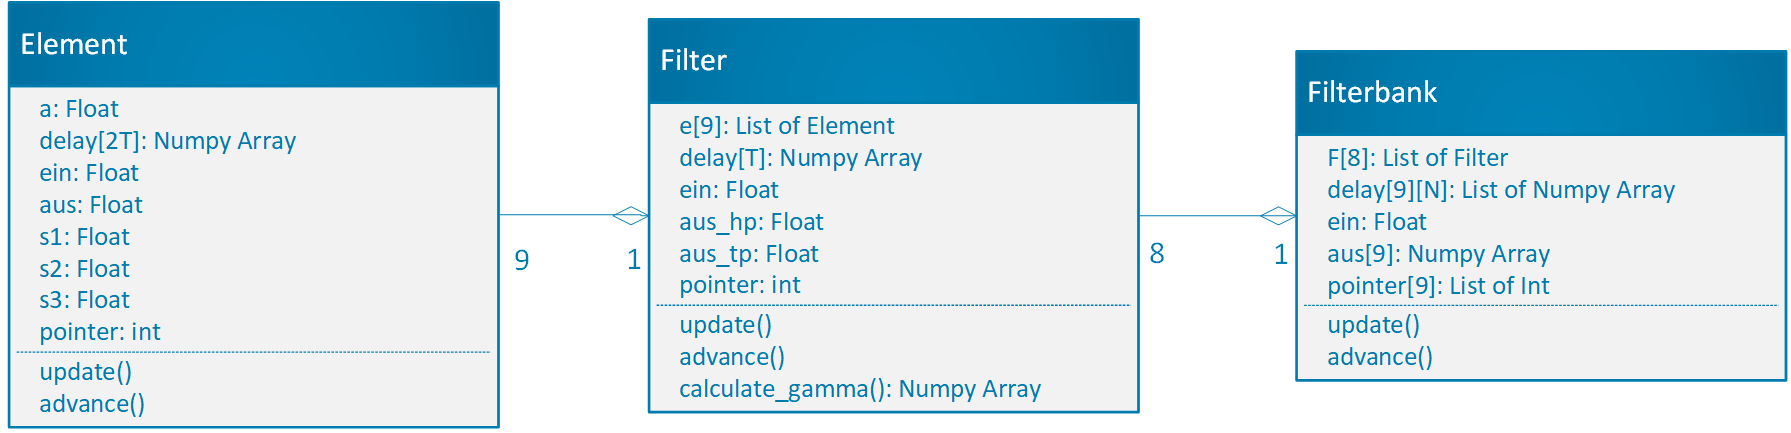
\includegraphics[width=1\textwidth]{img/klassendia}
  \caption{Klassendiagramm für die Implementierung einer hochselektiven Filterbank}\label{fig:impl_klassdia}
\end{figure}
Wie in Abbildung~\ref{fig:impl_klassdia} zu sehen erfolgt die Implementierung der hochselektiven Filterbank objektorientiert. Dabei besteht eine Filterbank aus 8 Filtern (vgl. Abb. TODO) und ein Filter aus 9 Elementen (vgl. Abb.).
\subsection{Klassen}\label{sec:impl_klassen}
Im folgenden wird die Implementierung der Klassen im einzelnen beschrieben bevor im nächsten Unterkaptitel auf dei verwendeten Testfunktionen eingegangen wird.
\subsubsection{Element}\label{sec:impl_ele}
Ein Element (s. Lst.~\ref{lst:element}) stellt den kleinsten Teil der Filterbank dar. Neben Ein- und Ausgang verfügt ein Element über ein Delay-Array dessen Länge bei der Initialisierung übergeben werden kann. Hierüber lässt sich die Ordnung des Teilfilters einstellen (vlg. Kap. TODO). Außerdem muss bei der Initialisierung ein Wert für \emph{a} übergeben werden. Dieser bestimmt mit welchem Wert im Element multipliziert wird (vlg. Abb. TODO).

Über das Aufrufen der Funktion \emph{update()} werden die Summen und der Ausgang des Elements neu berechnet. Die Funktion \emph{advance()} wird verwendet um einen Takt des Systems zu simulieren. Der Pointer, welcher den aktuellen Eingang des Verzögerungsgliedes anzeigt wird inkrementiert und ein neuer Wert wird in das Array geschrieben. Der aktuell gültige Augang des Verzögerungsarrays befindet sich eine Stelle \emph{vor} dem Eingang (vgl. Lst.~\ref{lst:element} Zeile 16).

\lstinputlisting[language=Python, firstline=6, lastline=31, caption={Quellcode der Klasse Element}, label={lst:element}]{list/wellendigitalfilter.py}


\subsubsection{Filter}\label{sec:impl_Filter}
Ein Teilfilter (s. Lst.~\ref{lst:filter}) besteht aus 9 Elementen und einem Verzögerungsglied (vlg. Abb. TODO). Bei der Initialisierung muss kann die Anzahl der Verzögerungen und damit die Ordnung des Teilfilters übergeben werden. Die Koeffizienten der Elemnte gemäß~\cite{gaszi1983} über die Funktion \emph{calculate\_gamma(fs, F)} berechnet. Wobei \emph{F} die Taktfrequenz des Systems und \emph{fs} die gewünschte Stopfrequenz des Filters ist.

Über die Funktion \emph{update()} werden die Ausgänge der enthaltenden Elemente nacheinander berechnet. Dabei wird dem Eingang der Ersten zwei Elemente der Wert des Filtereingangs zugewiesen. Die restlichen Eingänge ergeben sich durch die Augänge der vorherigen Filter. Durch die Funktion \emph{advance()} wird wieder der Takt simuliert. Die Verzögerungsglieder der Elemente und das Verzögerungsglied des Filters (vgl. Abb. TODO rechts) werden aktuallisiert.

\lstinputlisting[language=Python, firstline=34, lastline=118, caption={Quellcode der Klasse Filter}, label={lst:filter}]{list/wellendigitalfilter.py}

\subsubsection{Filterbank}\label{sec:impl_bank}
Die oberste Hierarchieebene bildet die Klasse Filterbank (s. Lst. \ref{lst:bank}). Sie beinhaltet die 8 Teilfilter (vlg. Abb. TODO). Als Ausgänge stehen die 9 Teilbänder zur verfügung. Diese sind um jeweils so verzögert, dass das Maximum der Impulsantworten der einzelnen Teilbänder in etwa zum gleichen Takt ausgegeben werden. Die Bestimmung dieser Verzögerungen erfolgte durch simulieren der Filterbank \emph{ohne} Anpassung der Laufzeiten. Dabei wurden die Maxima der Impulsantworten graphisch bestimmt (s. Tab.~\ref{tab:filt_max}).

\begin{table}[!htpb]
  \centering
  \begin{tabular}{c | l | c}
    \toprule
    Ausgang&Frequenzbereich&Maximum der Impulsantwort (in Takten)\\
    \midrule
    0&$F/4\ldots F/8$&4\\
    1&$F/8\ldots F/16$&20\\
    2&$F/16\ldots F/32$&44\\
    3&$F/32\ldots F/64$&91\\
    4&$F/64\ldots F/128$&186\\
    5&$F/128\ldots F/256$&375\\
    6&$F/256\ldots F/512$&755\\
    7&$F/512\ldots F/1024$&1500\\
    8&$F/1024\ldots F/2048$&900\\
    \bottomrule
  \end{tabular}
  \caption{Maxima der Impulsantworten der Teilbänder. \emph{F} entspricht der Taktfrequenz des Systems.}
  \label{tab:filt_max}
\end{table}
Damit ergeben sich die benötigten Verzögerungen gemäß Listing~\ref{lst:verz}.

\lstinputlisting[language=Python, firstline=249, lastline=253, caption={Quellcode zur Berechnung der zum Laufzeitausgleich benötigten Verzögerungen}, label={lst:verz}]{list/wellendigitalfilter.py}

Über die Funktion \emph{update()} werden die Eingänge der einzelnen Filter aktuallisiert und die Ausgänge berechnet. Die Simulation des Taktes erfolgt wieder über die Funktion \emph{advance()}. Es werden die Verzögerungsglieder aller Teilfilter und damit aller Elemente sowie die Verzögerungsglieder für den Laufzeitausgleich der Filterbank aktuallisiert.

\lstinputlisting[language=Python, firstline=121, lastline=160, caption={Quellcode der Klasse Filterbank}, label={lst:bank}]{list/wellendigitalfilter.py}
\subsection{Testfunktionen}\label{sec:impl_test}

\subsubsection{Test Filter}\label{sec:impl_testFilter}
Über die Funktion \emph{test\_Filter()} kann ein einzelner Teilbandfilter getestet werden. Hierfür wird die Impulsantwort des Teilbandfilters berechnet. Diese wird anschließend im Zeit- und Frequenzbereich dargestellt.
\lstinputlisting[language=Python, firstline=163, lastline=193, caption={Quellcode der Testfunktion für einen einzlnen Filter}, label={lst:test_filter}]{list/wellendigitalfilter.py}
\subsubsection{Test Filterbank}\label{sec:impl_testBank}
Die Funktion \emph{test\_Filter\_Bank()} wird verwendet um die gesamte Filterbank zu simulieren. Es wird ebenfalls die Reaktion auf einen Impuls berechnet. Anschließend werden die einzelnen Teilbänder sowie die Summe der Teilbänder im Frequenz- und Zeitbreich dargestellt.
\lstinputlisting[language=Python, firstline=196, lastline=244, caption={Quellcode der Testfunktion für die gesamte Filterbank}, label={lst:test_bank}]{list/wellendigitalfilter.py}
%%% Local Variables:
%%% mode: latex
%%% TeX-master: "../termpaper"
%%% End:
